\documentclass[a4paper,12pt,french]{article}

\usepackage{../../Style}

\renewcommand\tabularxcolumn[1]{m{#1}}

\renewcommand{\baselinestretch}{1.25}

\newcommand{\telepherique}[3] {
\path [fill=black, fill opacity=0.3, draw=black, line width=2pt ] (#1,#2) -- (#1+1,#2+1) -- (#1+2,#2) -- (#1+8,#2+2) -- (#1+4,#2-2) -- (#1+7,#2-5) -- (#1+4,#2-4) -- (#1+3,#2-6) node[color=black,circle,minimum size=1pt,fill,inner sep=2pt,fill opacity=1] {} node[below right,fill opacity=1] {\textbf{{\Large{#3}}}} -- (#1+3,#2-3) -- (#1+1,#2) -- (#1,#2);
}

\pagestyle{empty}

\begin{document}
 
\begin{center}
\textbf{\huge{ Activité - Vecteurs du plan }}
\end{center} 

\begin{center}
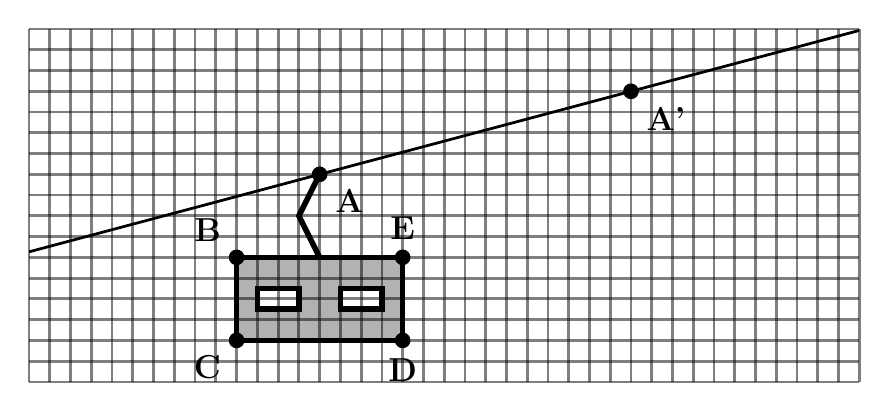
\begin{tikzpicture}[scale=1]
\begin{axis}[
%axis x line=bottom,
%axis y line = left,
%axis lines=middle,
width=\linewidth,
height=0.5\linewidth,
xmin=-5, xmax=17,
ymin=-10, ymax=7,
%enlargelimits={abs=0.2},
xtick distance=1,
ytick distance=1,
grid=both,
xticklabels={},
yticklabels={},
grid style={black,line width=1pt, draw opacity=0.5},
ticks=none,
axis equal,
legend pos=north east,
axis line style={draw=none},
]
\path [draw=black, line width=2pt] (0,0) -- (-1,-2) -- (0,-4);
\draw[draw=black, fill = black, fill opacity = 0.3, line width=2pt, even odd rule] 
        (-4,-8) rectangle (4,-4) (-3,-6.5) rectangle (-1,-5.5) (1,-6.5) rectangle (3,-5.5);
\node[color=black,circle,minimum size=1pt,fill,inner sep=2pt,fill opacity=1,label={-45:\textbf{\large A}}] (A) at (0,0) {};
\node[color=black,circle,minimum size=1pt,fill,inner sep=2pt,fill opacity=1,label={-45:\textbf{\large A'}}] (A') at (15,4) {};
\node[color=black,circle,minimum size=1pt,fill,inner sep=2pt,fill opacity=1,label={135:\textbf{\large B}}] (B) at (-4,-4) {};
\node[color=black,circle,minimum size=1pt,fill,inner sep=2pt,fill opacity=1,label={-135:\textbf{\large C}}] (C) at (-4,-8) {};
\node[color=black,circle,minimum size=1pt,fill,inner sep=2pt,fill opacity=1,label={-90:\textbf{\large D}}] (D) at (4,-8) {};
\node[color=black,circle,minimum size=1pt,fill,inner sep=2pt,fill opacity=1,label={90:\textbf{\large E}}] (E) at (4,-4) {};
\draw[line width=1pt, shorten <= -10cm, shorten >= -10cm] (A) -- (A');
\end{axis}
\end{tikzpicture}
\end{center}

Une télécabine se déplace le long d'un cable représenté ici par la droite $(AA')$.

\begin{enumerate}

\item Représenter la télécabine lorsqu'elle atteint le point $A'$, et placer les nouveaux points $B',\ldots$
\item Tracer une flèche de couleur reliant $A$ à $A'$.
\item De même, tracer une flèche reliant $B$ à $B', \ldots$

\begin{center}
On dit que $B'C'D'E'$ est \textbf{l'image} de $BCDE$ par la \textbf{translation} qui transforme $A$ en $A'$.
\end{center}


\item Que peut-on dire de ces flèches?

Toutes ces flèches correspondent au même déplacement: On dit qu'elles représentent un même vecteur $\vec u$, et on note $\vec u = \vecc {AA'} = \vecc {BB'} = \ldots = \vecc {EE'}$.

On dit que $\vecc {AA'}, \ldots, \vecc {EE'}$ sont des représentants du vecteur $\vec u$.

$A$ est l'origine du vecteur $\vecc {AA'}$, et $A'$ est son extrémité.

On dit alors que $B'C'D'E'$ est \textbf{l'image} de $BCDE$ par la \textbf{translation} de vecteur $\vecc {AA'}$.

\item Dans chacun des cas, tracer l'image du polygone par la translation de vecteur $\vecc {AA'}$.

\compo[0.5]
{
\begin{center}
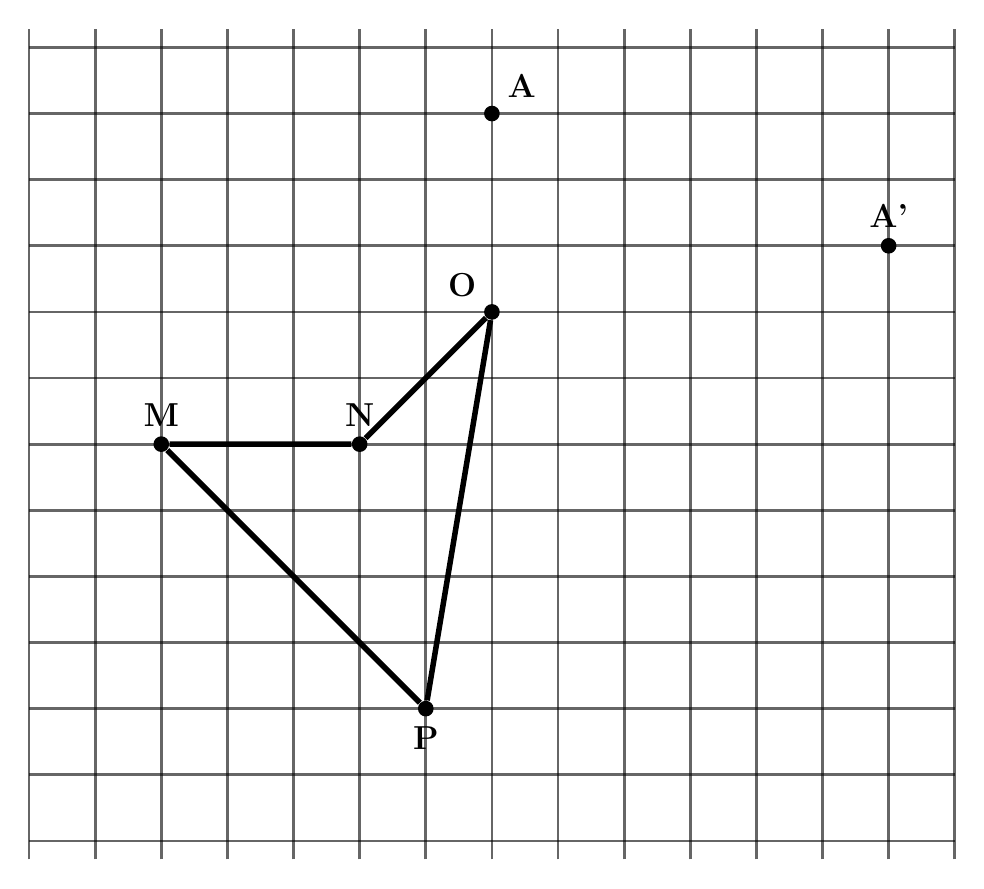
\begin{tikzpicture}[scale=1]
\begin{axis}[
%axis x line=bottom,
%axis y line = left,
%axis lines=middle,
width=1.1\linewidth,
height=\linewidth,
xmin=-2, xmax=12,
ymin=-5, ymax=5,
%enlargelimits={abs=0.2},
xtick distance=1,
ytick distance=1,
grid=both,
xticklabels={},
yticklabels={},
grid style={black,line width=1pt, draw opacity=0.6},
ticks=none,
axis equal,
legend pos=north east,
axis line style={draw=none},
]
\node[color=black,circle,minimum size=1pt,fill,inner sep=2pt,fill opacity=1,label={45:\textbf{\large A}}] (A) at (5,5) {};
\node[color=black,circle,minimum size=1pt,fill,inner sep=2pt,fill opacity=1,label={90:\textbf{\large A'}}] (A') at (11,3) {};
\node[color=black,circle,minimum size=1pt,fill,inner sep=2pt,fill opacity=1,label={90:\textbf{\large M}}] (M) at (0,0) {};
\node[color=black,circle,minimum size=1pt,fill,inner sep=2pt,fill opacity=1,label={-90:\textbf{\large P}}] (P) at (4,-4) {};
\node[color=black,circle,minimum size=1pt,fill,inner sep=2pt,fill opacity=1,label={135:\textbf{\large O}}] (O) at (5,2) {};
\node[color=black,circle,minimum size=1pt,fill,inner sep=2pt,fill opacity=1,label={90:\textbf{\large N}}] (N) at (3,0) {};
\draw[draw=black, fill = black, fill opacity = 0.3, line width=2pt, even odd rule] 
        (M) -- (N) -- (O) -- (P) -- (M);
\end{axis}
\end{tikzpicture}
\end{center}
}
{
\begin{center}
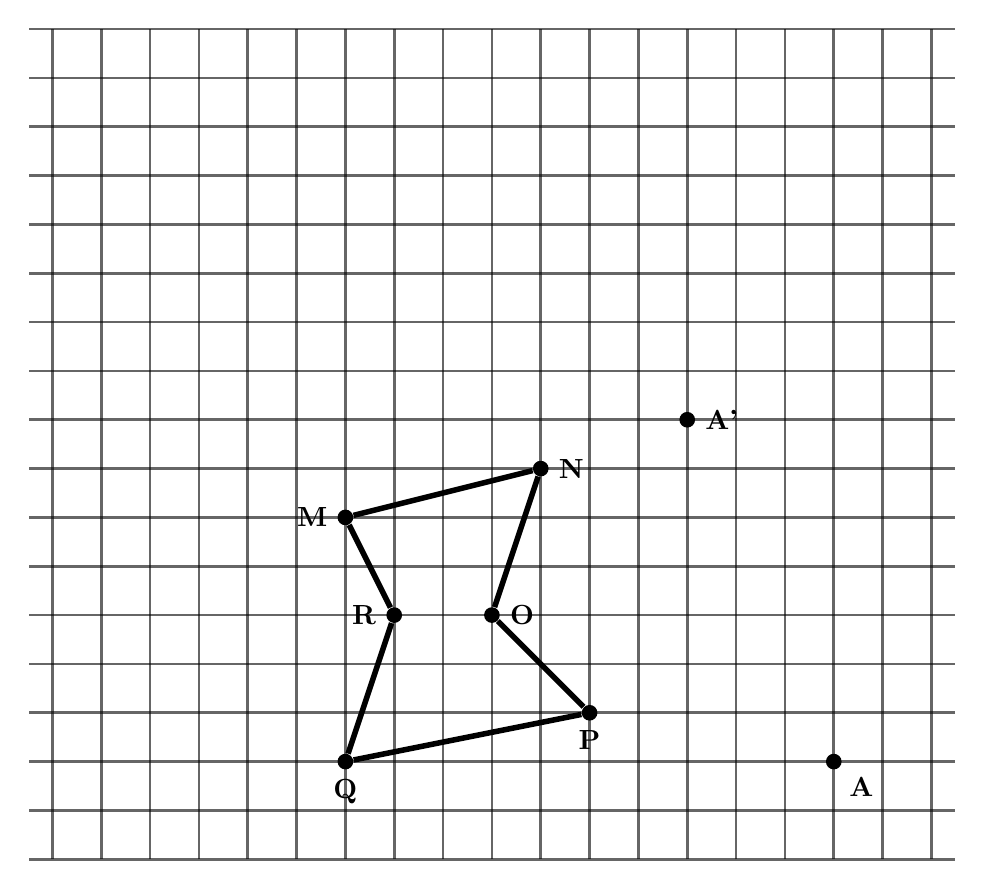
\begin{tikzpicture}[scale=1]
\begin{axis}[
%axis x line=bottom,
%axis y line = left,
%axis lines=middle,
width=1.1\linewidth,
height=\linewidth,
xmin=-4, xmax=10,
ymin=-7, ymax=10,
%enlargelimits={abs=0.2},
xtick distance=1,
ytick distance=1,
grid=both,
xticklabels={},
yticklabels={},
grid style={black,line width=1pt, draw opacity=0.6},
ticks=none,
axis equal,
legend pos=north east,
axis line style={draw=none},
]
\node[color=black,circle,minimum size=1pt,fill,inner sep=2pt,fill opacity=1,label={-45:\textbf{A}}] (A) at (10,-5) {};
\node[color=black,circle,minimum size=1pt,fill,inner sep=2pt,fill opacity=1,label={0:\textbf{A'}}] (A') at (7,2) {};
\node[color=black,circle,minimum size=1pt,fill,inner sep=2pt,fill opacity=1,label={180:\textbf{M}}] (M) at (0,0) {};
\node[color=black,circle,minimum size=1pt,fill,inner sep=2pt,fill opacity=1,label={-90:\textbf{P}}] (P) at (5,-4) {};
\node[color=black,circle,minimum size=1pt,fill,inner sep=2pt,fill opacity=1,label={0:\textbf{O}}] (O) at (3,-2) {};
\node[color=black,circle,minimum size=1pt,fill,inner sep=2pt,fill opacity=1,label={0:\textbf{N}}] (N) at (4,1) {};
\node[color=black,circle,minimum size=1pt,fill,inner sep=2pt,fill opacity=1,label={-90:\textbf{Q}}] (Q) at (0,-5) {};
\node[color=black,circle,minimum size=1pt,fill,inner sep=2pt,fill opacity=1,label={180:\textbf{R}}] (R) at (1,-2) {};
\draw[draw=black, fill = black, fill opacity = 0.3, line width=2pt, even odd rule] 
        (M) -- (N) -- (O) -- (P) -- (Q) -- (R) -- (M);
\end{axis}
\end{tikzpicture}
\end{center}
}

\end{enumerate}

\end{document}
